% This is samplepaper.tex, a sample chapter demonstrating the
% LLNCS macro package for Springer Computer Science proceedings;
% Version 2.21 of 2022/01/12
%
\documentclass[runningheads]{llncs}
%
\usepackage[T1]{fontenc}
% T1 fonts will be used to generate the final print and online PDFs,
% so please use T1 fonts in your manuscript whenever possible.
% Other font encondings may result in incorrect characters.

\usepackage{listings}
\usepackage{amsmath}

\usepackage{graphicx}
% Used for displaying a sample figure. If possible, figure files should
% be included in EPS format.
%
% If you use the hyperref package, please uncomment the following two lines
% to display URLs in blue roman font according to Springer's eBook style:
%\usepackage{color}
%\renewcommand\UrlFont{\color{blue}\rmfamily}
%\urlstyle{rm}

\usepackage{hyperref}


\usepackage{listings}
\usepackage{tcolorbox}
\usepackage{amsfonts}
\usepackage{todonotes}

\usepackage{subcaption}

\usepackage{orcidlink}

\usepackage[firstpage]{draftwatermark}


\definecolor{codegreen}{rgb}{0,0.6,0}
\definecolor{codegray}{rgb}{0.5,0.5,0.5}
\definecolor{codepurple}{rgb}{0.58,0,0.82}
\definecolor{codeyellow}{rgb}{0.67,0.67,0.0}
\definecolor{backcolour}{rgb}{0.96, 1.0, 0.98}
\definecolor{white}{rgb}{1.0,1.0,1.0}
\definecolor{codeblue}{rgb}{0,0,1.0}
\definecolor{darkred}{rgb}{0.59,0,0}
\definecolor{darkgreen}{rgb}{0,0.59,0}
\definecolor{yellow}{rgb}{0.87,0.85,0}
\definecolor{cyan}{rgb}{0,0.76,0.87}

\def\smalltext{\begingroup\scriptsize}
\def\endsmalltext{\endgroup}


\lstdefinestyle{mystyle}{
    backgroundcolor=\color{backcolour},   
    commentstyle=\color{codegreen},
    keywordstyle=[1]\color{magenta},
    keywordstyle=[2]\color{codeblue},
    keywordstyle=[3]\color{darkred},
    keywordstyle=[4]\color{darkgreen},
    keywordstyle=[5]\color{cyan},
    numberstyle=\tiny\color{codegray},
    stringstyle=\color{codepurple},
    basicstyle=\ttfamily\footnotesize,
    breakatwhitespace=false,         
    breaklines=true,                 
    captionpos=b,                    
    keepspaces=true,                 
    %numbers=left,
    numbers = none,
    numbersep=5pt,                  
    showspaces=false,                
    showstringspaces=false,
    showlines=true,
    showtabs=false,                  
    tabsize=2
}

\lstset{style=mystyle}

\lstdefinelanguage{yoda}{
    morekeywords=[1]{param,const, state, agent, features,  system, predicate, actions, behaviour, when, orwhen, otherwise, observations, bool, int, real, end, environment, sensing, <-, any, it, dynamic, element, configuration, for, sampled, distinct, time, from, do, endfor, measure, mean, let, and, endlet, in, if, else, endif},
    keywords=[2]{goIdle,read,send,save,turnOff,moveFromHall,moveToHall,moveFromCorridor,moveToCorridor, stop },
    keywords=[3]{status,batteryPerc,batteryCapacity,saving,registeredIAQ,savedCO2,minutes,movingTowards,sojournTime},
    keywords=[4]{lowChargeLed,numOfRoom,roomCO2,roomPos},
    keywords=[5]{numOfHuman,registeredCO2,isCrowded,currentRoom},
    sensitive=false, % keywords are not case-sensitive
    %morecomment=[l]{//}, % l is for line comment
    morecomment=[s]{/*}{*/}, % s is for start and end delimiter
    morestring=[b]" % defines that strings are enclosed in double quotes
} %

\lstdefinelanguage{traceSibilla}{
    morekeywords={x, y, z, direction, shape, colour, when, otherwise, blue, red, green, yellow, black, cyan, gray, magenta, white,  circle, square, triangle, hexagon, car, ant, bird},
    sensitive=false, % keywords are not case-sensitive
    morecomment=[l]{//}, % l is for line comment
    morecomment=[s]{/*}{*/}, % s is for start and end delimiter
    %morestring=[b]" % defines that strings are enclosed in double quotes
} %

\lstdefinelanguage{shellSibilla}{
    morekeywords={modules, module, load, env, environment, set, clear, reset, states, init, replica, deadline, dt, measures, add, all, remove, measure, remove, save, output, prefix, postfix, run, quit, simulate, trace, in},
    sensitive=false, % keywords are not case-sensitive
    morecomment=[l]{//}, % l is for line comment
    morecomment=[s]{/*}{*/}, % s is for start and end delimiter
    %morestring=[b]" % defines that strings are enclosed in double quotes
} %



% Sibilla population odel keyword

\lstdefinelanguage{populationLang}{
    morekeywords={param,const, species, rule, |,  -[ , ]-> , system, predicate},
    sensitive=false, % keywords are not case-sensitive
    morecomment=[l]{//}, % l is for line comment
    morecomment=[s]{/*}{*/}, % s is for start and end delimiter
    morestring=[b]" % defines that strings are enclosed in double quotes
} %

\lstdefinelanguage{LIOLang}{
    morekeywords={param,const, species, rule, |,  -[ , ]-> , system, predicate, state, endstate, action},
    sensitive=false, % keywords are not case-sensitive
    morecomment=[l]{//}, % l is for line comment
    morecomment=[s]{/*}{*/}, % s is for start and end delimiter
    morestring=[b]" % defines that strings are enclosed in double quotes
} %

\lstdefinelanguage{slam}{
    morekeywords={param,const, state, agent, features,  system, predicate, actions, behaviour, when, orwhen, otherwise, observations, bool, int, real, end, environment, sensing, <-, any, it, dynamic, attributes, rnd, PI, views, exists, boolean, init, after, if, else, send, on, time, states, now, dt, cos, sin, U},
    sensitive=false, % keywords are not case-sensitive
    morecomment=[l]{//}, % l is for line comment
    morecomment=[s]{/*}{*/}, % s is for start and end delimiter
    morestring=[b]" % defines that strings are enclosed in double quotes
} %


\newcommand{\yoda}{\textsf{YODA}}
\newcommand{\sibilla}{\textsf{Sibilla}}

%
\begin{document}
\SetWatermarkText{\hspace*{3.7in}\raisebox{8.55in}{\href{https://eapls.org/pages/artifact_badges/}{\mbox{
\includegraphics[width=1.4cm]{badges/available}
\includegraphics[width=1.4cm]{badges/reusable.png}}}}} 
\SetWatermarkAngle{0}
%
%\title{Simulating and Analysing Battery Life and Coverage of a Group of Air Quality-Measuring Devices with YODA}
\title{Simulation and Analysis of Indoor-Air-Quality Measuring Devices with YODA\thanks{This paper has been partially supported by the project SIMBA, funded by Regione Marche under the initiative ``Dottorati Innovativi'' (CUP B14E24001160009).}}

%
\titlerunning{Simulation and Analysis of IAQ Measuring Devices with YODA}
% If the paper title is too long for the running head, you can set
% an abbreviated paper title here
%
\author{Riccardo Petracci\orcidlink{0009-0009-1984-6317} 
\and Nicola {Del Giudice}\orcidlink{0000-0002-5194-0823}
\and Diletta Romana Cacciagrano\orcidlink{0000-0003-4491-0666}
\and Michele Loreti\orcidlink{0000-0003-3061-863X}
}
%
\authorrunning{R. Petracci et al.}
% First names are abbreviated in the running head.
% If there are more than two authors, 'et al.' is used.
%
\institute{University of Camerino, Via Madonna delle Carceri 9, Camerino, 62032, Italy\\
\email{\{riccardo.petracci, nicola.delgiudice, diletta.cacciagrano, michele.loreti\}@unicam.it}
}
%
\maketitle              % typeset the header of the contribution
%
\begin{abstract}
Collective Adaptive Systems (CAS) are groups of heterogeneous components that interact to achieve local and global goals.
%
One way to view CAS is to consider them as intelligent agents that operate according to a behaviour based on observations and a state.
%
%In the last year, many formalisms have been proposed to support the specification and analysis of CAS. 
%
Internet-of-Things (IoT) ecosystems provide a natural application domain for agent-based solutions to support modelling and analysis, as they share many architectural similarities. 
%
In this paper, we show how one of the recently proposed agenda-based languages, named \yoda{}, can be used to support the design and engineering of an IoT system designed to measure indoor air quality and warn if it falls below a given threshold.
%
The proposed model has been simulated using the tool \sibilla{} to forecast how battery life, coverage, and overall Indoor Air Quality evolve with the number of people in a building.
%
%For our means, we use the \yoda{} multi-agent language and the \sibilla{} forecasting tool. These two solutions provide a good level of abstraction, which is useful while designing the IoT ecosystem.
%
In the paper, we show how the proposed methodology can be used during the design phase to support developers and engineers and aid their decision-making, without relying on real-world deployment.
%
\keywords{Collective Systems \and Multi-Agent Systems \and IoT \and Indoor Air Quality}
\end{abstract}
%
%
%
\section{Introduction}\label{sec:intro}

Collective Adaptive Systems (CAS)~\cite{holzl2008engineering} are defined as groups of heterogeneous components that interact with each other and the surrounding environment to achieve local and global goals.
%
In this kind of system, components act without centralised control, and their behaviour adapts to changes in the surrounding environment.
%
As interactions among components can become intricate, it is crucial to understand how these components evolve over time.
%
Under these circumstances, we need to use rigorous methodologies and tools to specify and simulate CAS and verify their correct functioning.

One way to see CAS is to consider them as groups of \emph{agents}, or, to be more precise, \emph{intelligent agents}~\cite{wooldridge1995intelligent}. These computational entities can support complex interactions and adapt their behaviour as the whole system evolves.
%
If these agents operate and interact with each other, we are considering a Multi-Agent System (MAS)~\cite{Rocha17,wooldridge2009introduction,stone2000multiagent}, which is defined as ``\emph{a loosely coupled network of problem-solving entities (agents) that work together to find answers to problems that are beyond the individual capabilities or knowledge of each entity (agent)}''.

Internet-of-Things (IoT) ecosystems provide a natural playground for working with MAS. As IoT systems rely on the three layers of Perception, Network, and Application, it is natural to think of them as agent-based systems. 
%
Many examples of this union can be found in the literature, spanning from smart home environments~\cite{HarrabiHAZ24} to smart cities~\cite{nezamoddini2022survey} or smart manufacturing~\cite{alzubaidi2024multi}. MAS can also help understand and predict how energy behaves and evolves over time through distributed communication and control. Specifying and simulating such systems in a digital environment can help us optimise real ones, without wasting important resources~\cite{gonzalez2018multi,sadeeq2021design}.


In this paper, we analyse the evolution of a smart ecosystem considering a set of IoT devices and different people walking around. In this scenario, the devices analyse the Indoor Air Quality (IAQ), which is influenced by the number of people around each device. 
%
Devices can identify people and measure carbon dioxide levels in a room. As in \sibilla{}, the system evolves at fixed times, and agents operate synchronously, at every scheduled time, the device reads the CO$_2$ levels and calculates the IAQ.
%
%If the IAQ level from the previous measurement falls below a given threshold, or if there are too many people in a room, the timer is ignored to read the air quality and the data is later sent to a hypothetical server.
%
The goal of this paper is to develop a model that can forecast system behaviour to measure parameters such as each device's battery life, changes in area coverage over time due to people movement, and the general IAQ index.

The proposed model mimics a real part of a university building, abstracted into nine equal-sized rooms with low ventilation. These are organised into a main hall connected to five rooms and a secondary hall connected to three rooms and to the main hall itself.
%
IAQ is modelled exclusively through CO$_2$ concentration, and each device operates according to a timer-based strategy. They read at regular intervals, but they are also forced whenever a person enters a room or when the IAQ index drops below a given critical threshold. 
%
%Under a given threshold, the sampling frequency is increased. 
%
The dynamic activation and deactivation of devices are governed by an adaptive mechanism that considers the number of people in the room and the IAQ index, allowing the system to balance battery consumption and to analyse the percentage of devices not in energy-saving mode.
%
The entire ecosystem is modelled leveraging the \yoda{}~\cite{yoda} MAS language and simulated with the \sibilla{}~\cite{sibilla} forecasting tool. Different scenarios are evaluated by varying the number of people across rooms and the IAQ threshold values to assess their impact on device lifetime, coverage, and air quality.

The main goal of the paper is to present a methodology for use during the design phase of an IoT ecosystem.
%
As we will see later in Section~\ref{sec:related}, many methods are based on technical deployment and specific cases.
%
Instead, our approach aims to provide simulation results that inform early decision-making processes, where it is fundamental to make architectural and system choices.
%
In fact, the ultimate objective of this research is to provide a methodology, through an experiential approach, for critically analysing the evolution of an IoT environment. This methodology can enable developers and engineers to implement resources without wasting either resources or time.

The remainder of the paper is structured as follows.
%
In Section~\ref{sec:related}, we review some similar works and how they deal with MAS and IoT.
%
Section~\ref{sec:background} introduces the tools used to develop the presented approach.
%
In Section~\ref{sec:spec}, the actual specification of the proposed case study is presented.
%
Section~\ref{sec:sim} presents the simulation of our IoT system and discusses the results.
%
Finally, we conclude the paper with some remarks for future iterations in Section~\ref{sec:conc}.
%

\section{Related Works}\label{sec:related}

As IoT systems become increasingly prevalent in our lives, it is crucial to provide methods for modelling such systems and analysing the resulting data. An example is the \emph{ACOSO} framework~\cite{FortinoRSSZ18}, where all smart objects are modelled as agents that run across three architectural layers. Agents operate across the application, transport, and network/physical layers, interacting directly with sensors, actuators, and networking components. Here, the authors emphasise the system's design and implementation, leaving aside its macro-level emergent properties. This decision implies that each object (or agent) must handle its own resource management and communication, and that if an ecosystem increment becomes large, the number of agents and the complexity of their interfaces increase significantly.

\emph{FIoT}~\cite{NascimentoL17} is an example of a MAS-based framework for developing an IoT application that can self-adapt and self-organise. This framework combines MAS agents and machine learning techniques such as neural networks and evolutionary algorithms. 
%
The authors demonstrate the framework's practical application through two real-world scenarios: Quantified Things (i.e., smart agriculture) and self-organising smart street lights, using neuronal algorithms to enable autonomous decision-making.
%
Compared with our approach, this framework includes the concept of different agents and device roles. 
%
They still require engineers to define and tune agents for devices, controllers, and learning algorithms. 
%
In contrast, the present proposal operates at an aggregate level with greater abstraction capabilities, able to take global properties, thus avoiding complexity and scalability limitations.

Brandão et al.~\cite{BrandaoLPZV21} present an approach based on Belief-Desire-Intention (BDI) agents and the JaCaMo framework. JaCaMo~\cite{BoissierBHRS13} is a platform for developing MAS that integrates three key programming dimensions called \emph{Ja}son (agents), \emph{Ca}rtago (environment), and \emph{Mo}ise (organisation). The combination of BDI and JaCaMo introduces multiple agents that must manage hardware, such as sensors and actuators, as well as communication and general tasks. In this way, they do not prefer the server placement, but the hardware interfaces, message formats, and edge. 
%
The solution proposed by Brandão et al. involves compromises and highlights bottlenecks. The abstraction presents problems related to the growth in complexity with increasing device count, because there is a correlation between the agent and the device that creates an agent-per-device granularity.

The approach presented by Dähling et al. in~\cite{DahlingRM21} highlights the problem of building large-scale, fault-tolerant MAS in the IoT, where this scenario is often characterised by thousands or even millions of devices. 
%
They present a modern multi-agent platform based on cloud-computing techniques to solve the problem. The solution does not raise the modelling abstraction, as agents still represent individual devices or services that interact via message passing.
%0
The approach of~\cite{DahlingRM21} requires specifying agents for each sensor or actuator, along with their respective communication protocols. Aspects related to network configuration management and implementation should also be specifically modelled. This lacks abstract modelling capable of combining all system components and considering possible increases in the number of agents per device in large-scale ecosystems.

Some examples focused on behaviour and the formal modelling of IoT environments can be considered high-level. The approach used by Batool et al. is based on Cognitive Agent-Based Computing (CABC)~\cite{BatoolN17} and proposes a framework for simulating complex IoT networks. To model the environment, they combine complex networks and agent-based models where agents represent nodes in topologies and are used to study network-level properties. The authors argue that packet-level simulators are not suitable for large IoT environments, so they motivate the need for an agent-based model as a high-level alternative. However, the abstraction of this approach links an agent to a node, and there is no aggregation or language based on the field that can collect behaviour information.

Another approach is based on the Bigraphical Agent (BiAgent)~\cite{MarirKBB17}, which aims to define a model for IoT applications. This model has been developed to support the structural aspects of IoT application modelling. Additionally, the model incorporates agents responsible for specifying analytics and decision-making aspects.
%
In their work based on the BiAgents model, Souad M. et al.~\cite{SouadFN20} propose a formal description of the structure and behaviour of IoT systems. Additionally, the specification is encoded into the Maude language, thereby facilitating the automatic execution of behaviours intrinsic to IoT systems. 
%
Using BiAgents and rewriting logic to provide a formal description of the IoT structure yields a mathematically precise and executable model, but the modeller controls the explicit structure and rules. However, like others, this work lacks a macro-programming perspective on global collective behaviours.

The gap that emerges with the existing works is that existing MAS and IoT frameworks excel at engineering and deployment, but they need a modeller who thinks about single agents (or devices). The low-level granularity also makes scalability challenging. 
%
Regarding agent-based models for IoT, the abstraction is raised above the packet and hardware levels, but there is no collective high-level or aggregate language. They treat agents (nodes) explicitly, without tailoring to IoT properties such as spatial coverage or battery evolution across a large population.

%%%%%%%%%%%%%%%%%%%%%%%%%%%%%%%%%%%%%%%%%%%%%%%%%%%%%%%%%%%%%%%%%%%%%%%%%%%%%%%%%%%%%%%%%%
%%%%%%%%%%%%%%%%%%%%%%%%%%%%%%%%%%%%%%%%%%%%%%%%%%%%%%%%%%%%%%%%%%%%%%%%%%%%%%%%%%%%%%%%%%
%%%%%%%%%%%%%%%%%%%%%%%%%%%%%%%%%%%%%%%%%%%%%%%%%%%%%%%%%%%%%%%%%%%%%%%%%%%%%%%%%%%%%%%%%%
\section{A short introduction of \yoda{} and \sibilla{}}\label{sec:background}
%%%%%%%%%%%%%%%%%%%%%%%%%%%%%%%%%%%%%%%%%%%%%%%%%%%%%%%%%%%%%%%%%%%%%%%%%%%%%%%%%%%%%%%%%%
%%%%%%%%%%%%%%%%%%%%%%%%%%%%%%%%%%%%%%%%%%%%%%%%%%%%%%%%%%%%%%%%%%%%%%%%%%%%%%%%%%%%%%%%%%
%%%%%%%%%%%%%%%%%%%%%%%%%%%%%%%%%%%%%%%%%%%%%%%%%%%%%%%%%%%%%%%%%%%%%%%%%%%%%%%%%%%%%%%%%%

To design and predict the behaviour of CAS systems, we need tools that allow researchers to specify that behaviour. An ideal candidate for this task is the \yoda{}~\cite{yoda} framework. 
%
\yoda{} is an agent-based specification language developed for describing the behaviour of computational entities based on possible actions that can be performed.
%
\yoda{} allows us to interact with and sense the surrounding environment, which is a fundamental aspect in the IoT context, especially when the main goal is to measure IAQ. In fact, this task is more difficult to achieve with tools like Actor Models, because they rely on messages rather than actively sensing the environment.
%
The language is equipped with a computational model that defines how each component of \yoda{} interacts with the others.
%
In a \yoda{} model, we need to define three elements: 1) the types of \emph{agents} operating in the system, 2) the \emph{environment} where the agents operate, and 3) the possible \emph{initial configurations}.
%
An agent is defined in terms of observations and state, which in turn is divided into internal state, defining attributes known only to the agent, and features, defining environmental attributes.
%
The agent operates by selecting one of the available actions based on its internal state and the observations gathered from the environment. Upon selecting an action, the agent's internal state is updated accordingly.
%
A key feature of \yoda{} is the possibility to model the enclosing environment.
% and give it specific responsibilities.
%
The latter is responsible for informing agents about what they can observe and updating their feature attributes. The latter are updated according to the performed action.
%
In this way, we can model even agent mobilities and possible interactions with IoT devices, which have their own spatial characteristics.
%
To make these concepts explicit, a specification language has been developed. This is a high-level language for describing MAS according to the \yoda{} paradigm, which has been used to design the IAQ-measuring ecosystem described in this paper.



To simulate and analyse our scenario, we use the \sibilla{}~\cite{sibilla} simulation tool. 
%
\sibilla{} is a Java tool for simulating Collective Systems. 
%
The tool has been conceived as modular software that serves as a container for different specification formalisms, allowing us to overcome the limitations of language-based tools.
%
In fact, the key feature of \sibilla{} is its customizability. Indeed, it is already equipped with a set of languages to design collective systems, such as \yoda{}, and other specification languages can be integrated.
%
The tool is also equipped with APIs for 1) \emph{simulating systems}, thus forecasting systems' behaviour, 2) \emph{performing transient analysis} to prove correctness of models via statistical model checking, and 3) \emph{modelling different CASs}, to define various types of systems.
%
This choice allows us to provide an even more abstract solution that simulates complex IoT scenarios during the design phase, helping IoT ecosystem designers make preliminary choices about how to arrange the devices.



%%%%%%%%%%%%%%%%%%%%%%%%%%%%%%%%%%%%%%%%%%%%%%%%%%%%%%%%%%%%%%%%%%%%%%%%%%%%%%%%%%%%%%%%%%
%%%%%%%%%%%%%%%%%%%%%%%%%%%%%%%%%%%%%%%%%%%%%%%%%%%%%%%%%%%%%%%%%%%%%%%%%%%%%%%%%%%%%%%%%%
%%%%%%%%%%%%%%%%%%%%%%%%%%%%%%%%%%%%%%%%%%%%%%%%%%%%%%%%%%%%%%%%%%%%%%%%%%%%%%%%%%%%%%%%%%
\section{Modelling IoT for Indoor Air Quality}\label{sec:spec}

In this section, we present the rationale for the modelling of the proposed IAQ scenario. First, we described the scenario from a general point of view and explained how we abstracted some parameters. After, we enter the model specification, presenting respectively i) the parameters and constants, ii) the IAQ measuring devices specification, and iii) the human agents specification. Finally, we conclude the section with the system configuration, which is later used to initialise the agent during the simulation process.

\subsection{IAQ Scenario Abstraction}

The model we want to represent~\footnote{The whole model specification is available at \url{https://github.com/quasylab/sibilla/wiki/YODA\#indoor-air-quality}} depicts a type of dynamic interaction within embedded systems equipped with various types of sensors that form a distributed network.
%
The distributed network consists of nodes that interface with each other, and their behaviour is influenced by the stochastic behaviour of the $N$ human occupants within a room $R$. 

\begin{figure}
    \centering
    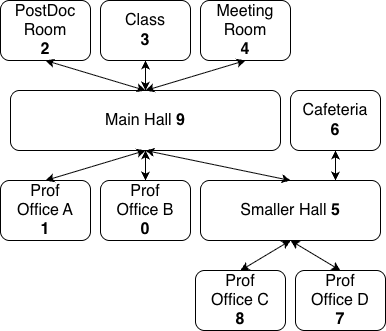
\includegraphics[width=0.4\linewidth]{University.png}
    \caption{Scheme of the University environment of our scenario}
    \label{fig:university}
\end{figure}

This type of model is used in simulation to analyse the system's ability to cope with, overcome, and reorganise its work and energy consumption. This means maintaining a constant work regime over time while providing adequate coverage of the area to be monitored, even in conditions of limited resources when nodes are shut down. 
%
The difference between this environment and classic statistical models lies in how the environment is treated. It is a living ecosystem in which the data recorded by the sensors is determined by human presence. 
%
In our scenario, we represent an abstraction of the university's room arrangement, as shown in Figure~\ref{fig:university}. 
%

The topological representation is a simplified model designed to mirror a real-world scenario within our institute. This topology is scalable and can be generalised to accommodate an arbitrary number of $N$ rooms. 
%
To maintain the consistency of the system logic, the \textit{Main Hall} and the \textit{Smaller Hall} must remain the central hubs to which all rooms are attached. The indexing convention is defined as follows:
%
\begin{itemize}
    \item \textbf{Main Hall (MH) Connections:} Rooms connected to the Main Hall are assigned indices ranging from $0$ to $nRoom_{MH} - 1$.
    \item \textbf{Smaller Hall (SH) Indexing:} The Smaller Hall itself is assigned the index $nRoom_{MH}$. The rooms connected to the Smaller Hall have indices ranging from $nRoom_{MH} + 1$ to $nRoom_{MH} + nRoom_{SH}$.
    \item \textbf{Main Hall Index:} The final index for the Main Hall is calculated as $Index_{MH} = nRoom_{MH} + nRoom_{SH} + 1$
\end{itemize}
%
This structure ensures that the core logic remains functional regardless of the total number of rooms added to the system.

%
The system works by detecting human presence and performing its tasks based on the “wake-on-demand” philosophy. Based on this philosophy, devices within a room remain in an idle state to consume less energy and only increase their activity when people are detected in the room, thanks to motion sensors~\cite{s24072123,jpmcj2019101037}. 
%
The device's energy efficiency takes a back seat when people are in the room, as the priority becomes controlling the air quality. For this reason, the device will have to work harder to monitor air quality data and send the data to the server, at the expense of increased energy consumption.
%
IAQ~\cite{s24216850} of a closed room is affected by different pollutants that can be correlated by human presence (i.e., CO$_2$, VOCs, PM2.5, PM10) and other pollutants not strictly related to their presence (i.e., CO, NH$_3$, NO2)~\cite{DasIN25,PREK2017228}. 
%
IAQ is critical for health, comfort, and productivity, as most of the population nowadays spends more than 80\% of their time indoors, and pollutants can be up to 5 times higher indoors than outdoors.
%
The low quality of indoor air can be hazardous to human health, causing symptoms such as headaches, allergies, and fatigue. 
%
On the other hand, maintaining good IAQ helps people enhance cognitive functions, improve sleep quality, and increase productivity in workplaces (e.g., schools, offices)~\cite{DasIN25}.

In general, the model specified in Section~\ref{subsec:iaqspec} is a self-organising environment in which IoT devices equipped with sensors can analyse the situation and perform different actions based on the information they retrieve. 
%
Functioning is subject to modification in response to human interaction with the environment. 
%
The interaction of humans with their environment begins with elementary movement or occupancy, and subsequently progresses to the introduction of a contaminant. Each human introduces pollutants into the rooms (abstracted as small offices) with scarce ventilation, so the air recycle is possible only when no humans are inside the room, thanks to the mass balance law~\cite{HERNANDEZCRUZ2026114099}.
    
\subsection{IAQ Scenario Parameters and Constants}\label{subsec:iaqparam}

To properly set up our scenario, we need to declare constants and parameters.
Concerning the first, we declare eight constants that represent the different devices' status through numerical values (\lstinline{idle}, \lstinline{reading}, \lstinline{sending}, \lstinline{battSave}, \lstinline{exhausted}), the minimum and maximum CO$_2$ that can be inside a room (\lstinline{CO2min} equals to 600 and  \lstinline{CO2max} to 3000), and the Nepero constant approximated with 3 decimal digits (\lstinline{nepero}).

For the parameters, we declare a set used to model the CO$_2$ concentration in a room, the devices, and the humans who sojourn in various rooms. The parameters \lstinline{CO2out} (outdoor CO$_2$), \lstinline{CO2ph} (average CO$_2$ produced by a human), and \lstinline{ventilation} (ventilation coefficient of the room) are used to compute the CO$_2$ concentration in a room.
%
We decided to perform our abstraction and simulation using only the CO$_2$ pollutant, as it is the most relevant parameter for calculating a general concentration. Using only this pollutant is reductive for a real scenario because to calculate the IAQ, we should also collect other information (i.e., VOC, NO$_x$, CH$_2$O, PM2.5, PM10, etc.), but performing these assumptions requires a higher effort, assuming real scenarios with different humans, possible external conditions, and indoor rooms characteristics.
%
The battery of devices loses percentage points based on activities done, which also affects the status, and to equalise the context, the consumption in \emph{mA} of all devices is parametrised (\lstinline{idleCons}, \lstinline{readCons}, and \lstinline{sendCons}). 
%
Two parameters (\lstinline{sendTimer} and \lstinline{readTimer}) regulate the duty cycle of a device that monitors air quality and sends information to the server. 
%
Another important parameter is the battery capacity (\lstinline{initMaxBatteryCapacity}), which helps determine which battery is most suitable to use. 
Since each simulation step represents one minute, the capacity, usually expressed in \emph{mAh} (milliampere-hours), is here expressed in mAmin (milliampere-minutes), where 1\emph{mA} is equivalent to 60\emph{mAmin} of cumulative discharge.

We declare different parameters to model human behaviour and orchestrate how they move between rooms. In a system, there are different humans (\lstinline{nHuman}) who have a sojourn time to stay in a room before moving to another one, and this is decided by randomly choosing between a minimum and maximum sojourn time (\lstinline{maxST}, \lstinline{minST}), making the movement of the various agents random. 
%
Moreover, two other parameters link the human behaviour and the device one, using two different thresholds (\lstinline{threshold}, \lstinline{minH}). It is possible to define how many humans can be accommodated in a room by a human, and the minimum number of humans required to activate the device's reading routine. This means that if there are too many people in a room, it is marked as crowded and they need to be moved to another room. 
%
With the other threshold, it is possible to regulate the device's sensitivity, which ignores the timer and instead analyses the air quality in the room.
%
To tweak the number of satellite rooms of the two halls, \lstinline{nSatellitesMainHall} and \lstinline{nSatellitesSmallHall} are used.

\subsection{IAQ Device Specification}\label{subsec:iaqspec}

Each agent \lstinline{Device} has to analyse the CO$_2$ inside the corresponding room.
%
From a general point of view, these agents sense the presence of people in the room and measure the level of carbon dioxide, thereby calculating the IAQ of the room.
%
If the IAQ is no longer acceptable, the \lstinline{Device} sends a message to a hypothetical server.
%
This process is repeated throughout the simulation, and when the battery is low, an alarm LED is activated. In the proposed example, humans can't replace the battery, and when it's drained, it simply turns off.
Listing~\ref{lst:deviceagent} shows the specification of said agent.

\begin{figure}[htbp!]
\begin{lstlisting}[language=yoda,basicstyle=\scriptsize, caption={IAQ Scenario: \textsf{Device} agent}, label={lst:deviceagent}]
agent Device =
  state:
    int status = 0;
    real batteryPerc = 100.0;
    real batteryCapacity = 10000.00;
    int saving = 1;
    real registeredIAQ = 100.0;
    real savedCO2 = 600.0;
    int minutes = 0;
  features:
    bool lowChargeLed = false;
    real numOfRoom = 0.0;               
    real roomCO2 = 600.0;
  observations:
    real numOfHuman = 0;     
    real registeredCO2 = 600.0;    
  actions:
    goIdle [
      status <- idle;
      batteryCapacity <- batteryCapacity - idleCons;
      batteryPerc <- 100 * (batteryCapacity - idleCons) / initMaxBatteryCapacity;
      registeredIAQ <- 100 * (CO2max - registeredCO2) / (CO2max - CO2min);
      savedCO2 <- registeredCO2;
      minutes <- minutes + 1;
    ]
    read [
      status <- reading;
      batteryCapacity <- batteryCapacity - (readCons + idleCons);
      batteryPerc <- 100 * (batteryCapacity - (readCons + idleCons)) / initMaxBatteryCapacity;
      registeredIAQ <- 100 * (CO2max - registeredCO2) / (CO2max - CO2min);
      savedCO2 <- registeredCO2;
      minutes <- minutes + 1;
    ]
    send [
      status <- sending;
      batteryCapacity <- batteryCapacity - (sendCons + idleCons);
      batteryPerc <- 100 * (batteryCapacity - (sendCons + idleCons)) / initMaxBatteryCapacity;
      registeredIAQ <- 100 * (CO2max - registeredCO2) / (CO2max - CO2min);
      savedCO2 <- registeredCO2;
      minutes <- minutes + 1;
    ]
    save [
      status <- battSave;
      saving <- 2;
      batteryCapacity <- batteryCapacity - idleCons;
      batteryPerc <- 100 * (batteryCapacity - idleCons) / initMaxBatteryCapacity;
      registeredIAQ <- 100 * (CO2max - registeredCO2) / (CO2max - CO2min);
      savedCO2 <- registeredCO2;
      minutes <- minutes + 1;
    ]
    turnOff [
      status <- exhausted;
      batteryCapacity <- 0;
      batteryPerc <- 0;
    ]
  behaviour:
    when batteryPerc <= 0 -> [turnOff:1;]
    orwhen (batteryPerc <= 30) && (saving == 1) -> [save:1;]
    orwhen (minutes%(sendTimer*saving)) == 0 -> [send:1;]
    orwhen ((minutes%(readTimer*saving)) == 0) || (numOfHuman>minH) || (registeredIAQ<85) -> [read:1;]
    otherwise [goIdle:1;]
end
\end{lstlisting}
\end{figure}


Regarding the internal state, we can include the \lstinline{status}, initialised to idle mode by default, and the \lstinline{batteryCapacity}, which is initially set to the parameter \lstinline{initMaxBatteryCapacity}. 
%
We also keep track of time passing with the \lstinline{minutes} attribute. 
%
With the \lstinline{saving} attribute, we manage the device's battery-saving status, which is used both as a multiplier and a controller. 
%
Indeed, it avoids setting the battery save status more than once, and when it is changed, it also acts as a multiplier, changing from 1 to another value (in our case, 2). This increases the time before performing actions that drain the battery more quickly, like sending a message.
%
Then we have to consider the indoor air quality, which is strictly related to CO$_2$ levels in a room. The \lstinline{registeredIAQ} represents the last IAQ index registered by the device, which reads the actual CO$_2$ (\lstinline{savedCO2}) in the room, and performs the formula. 
%
As features, we consider the physical LED of a device, which helps indicate when it is close to discharge. The use of the \lstinline{lowChargeLed} function indicates that the device has reached a percentage of 30\% or less. This configuration enables the device to enter a state of battery conservation, characterised by an increase in the time interval between scans or the time between data transmissions to the server.
%
We use the \lstinline{numOfRoom} to define the room where the device is located.
%
The CO$_2$ produced by a human is a feature in a room that is collected by a device to obtain the room's IAQ index.
%
Then, we can observe the number of humans present in the room (\lstinline{numOfHuman}) and the CO$_2$ registered by the device (\lstinline{registeredCO2}).

This agent has five different actions available for selection. Actions are responsible for changing an agent's state attributes. The first one is the \lstinline{goIdle}, which allows the agent to set the device in idle mode and calculate the remaining battery during this phase with low energy consumption (\lstinline{idleCons}). 
%
The battery capacity (\lstinline{batteryCapacity} and \lstinline{batteryPerc}) is calculated based on idle consumption parameters.
%
The \lstinline{read} and \lstinline{send} actions increase the device's battery consumption.
%
In the first one, a \lstinline{reading} status is established, and consumption increases due to sensor activation and the use of resources to monitor environmental pollution. 
%
In the other one, we set the device to the \lstinline{sending} status. Here, the consumption is higher due to the activation of communication protocols with the hypothetical server.
%
These actions have parameters (\lstinline{sendTimer}, \lstinline{readTimer}) that are analysed within the behaviour and help the agent manage the device's duty cycle. 
%
These two timers schedule how often the device must read data and send it to the server. It is also possible to configure these parameters to observe how agents' behaviour can change. 
%
The fourth action emulates a battery-saving status. It differs mainly from the other actions in that it changes the \lstinline{saving} attribute.
This attribute allows the agent to perform the \lstinline{save} action only once and to double the time required to perform the \lstinline{read} and \lstinline{send} actions.
%
Finally, the \lstinline{turnOff} action sets the device to \lstinline{exhausted} and the battery-related attributes are set to 0.
%
In general, all actions update the consumption based on three parameters (\lstinline{timeIdle}, \lstinline{timeRead}, \lstinline{timeSend}), which represent the estimated times the device takes to perform the various actions. The consumption considered with the parameters is an instantaneous average that must be averaged over time. 
%
When considering a one-minute time slice, we must bear in mind that the idle state lasts for 60 seconds, while the other actions last for the same amount of time as an idle state, but without the time required for reading or sending. This is because sensors and communication components consume the device's battery power only when they are in use, optimising battery consumption, not all the time.


Regarding the agent's behaviour, actions are performed based on the battery percentage and elapsed time, with a timer regulating the duty cycle of \lstinline{read} and \lstinline{send} actions.
%
The first check is on the battery: if the \lstinline{batteryPerc} is equal to 0, it means that the device is exhausted, but if the \lstinline{batteryPerc} is between 0 and 30, it means the device is close to exhausting the battery, and triggers the \lstinline{save} action.
%
Then it is checked whether sufficient time has passed to perform another sensor reading, or whether it is time to send data to the server.
%
If none of these rules is met, the \lstinline{goIdle} action is performed as the default action.
%
The behaviour of a device is deterministic, which means that, given the same conditions, the probability of doing the related action is 100\%.


\begin{figure}[htbp!]
\begin{lstlisting}[language=yoda,basicstyle=\scriptsize, caption={IAQ Scenario: \textsf{Device} Sensing and Dynamic Functions}, label={lst:deviceenv}]
environment:
  sensing:
    Device [
      let nh = #Human[roomPos == it.numOfRoom]
      and neperoK = nepero ^ ((-ventilation)/60)
      in
        numOfHuman <- nh;
        let newCO2  = CO2out+(((CO2ph*nh)/ventilation)*(1-neperoK))+                       ((roomCO2-CO2out)*neperoK)
        in
          if (newCO2 >= CO2min) then
            registeredCO2 <- newCO2;
          else
            registeredCO2 <- CO2min;
          endif
        endlet
      endlet
    ]
    ...
  dynamic:
    Device [
      lowChargeLed <- batteryPerc <= 30;
      roomCO2 <- savedCO2;
    ]
    ...
end
\end{lstlisting}
\end{figure}

The environmental updates of the \emph{Device}, which are listed in Listing ~\ref{lst:deviceenv}, allow us to change its observations and features. Within the sensing function, observations are recorded on the quantity of human presence and the registered levels of carbon dioxide. 
%
%Carbon dioxide is associated with human presence, and indoor air quality is influenced by this pollutant, as well as other pollutants, to avoid complexity in the system.
%
The CO$_2$ in a room is calculated considering a simplified concentration formula that requires parameters such as the Nepero number, the ventilation coefficient, the approximated carbon dioxide produced by a human, and the carbon dioxide already in that room.
%
Then, the features of the agent that represent the low battery charge level and the carbon dioxide in the room are computed within the \lstinline{dynamic} of the environment.





\subsection{Human Specification}\label{subsec:humaspec}
The behaviour of the \lstinline{Human} agent is modelled according to the rooms configuration seen in Figure~\ref{fig:university}.
%
Humans are directly responsible for the degradation of the air quality in a room, and their movement among available spaces is fundamental to understanding how quickly the batteries of IoT devices run out of energy. 
%
Moreover, we modelled the human agent to tolerate a given number of its similar in the same room: when the room is crowded (or its sojourn time has ended), the \lstinline{Human} moves to another room.


\begin{figure}[!htbp]
\begin{lstlisting}[language=yoda,basicstyle=\scriptsize, caption={IAQ Scenario: \textsf{Human} agent}, label={lst:humanagent}]
agent Human =
  state :
    real movingTowards = 0; int sojournTime = 10;
  features :
    real roomPos = 0.0;
  observations :
    bool isCrowded = false; real currentRoom = 0.0;
  actions :
    moveFromHall [movingTowards <- floor(U[0,(nSatellitesMainHall+1)]); sojournTime <- U[minST, maxST];]
    moveToHall [movingTowards <- (nSatellitesMainHall+nSatellitesSmallHall+1); sojournTime <- U[minST, maxST];]
    moveFromCorridor [movingTowards <- ceil(U[nSatellitesMainHall,(nSatellitesMainHall+nSatellitesSmallHall+1)]); sojournTime <- U[minST, maxST];]
    moveToCorridor [movingTowards <- nSatellitesMainHall; sojournTime <- U[minST, maxST];]
    stop [movingTowards <- currentRoom; sojournTime <- sojournTime - 1;]
  behaviour :
    when (isCrowded || (sojournTime<=0)) && (currentRoom == (nSatellitesMainHall+nSatellitesSmallHall+1)) -> [moveFromHall:0.90; stop:0.10;]
    orwhen (isCrowded || (sojournTime<=0))  && (currentRoom < nSatellitesMainHall) -> [moveToHall:0.90; stop:0.10;]
    orwhen (isCrowded || (sojournTime<=0)) && (currentRoom == nSatellitesMainHall) -> [moveFromCorridor:0.90; stop:0.10;]
    orwhen (isCrowded || (sojournTime<=0)) && ((currentRoom > nSatellitesMainHall) && (currentRoom<=8)) -> [moveToCorridor:0.90; stop:0.10;]
    otherwise [stop:1;]
end
\end{lstlisting}
\end{figure}

In Listing~\ref{lst:humanagent}, we display the specification of the \lstinline{Human} agent.
%
The agent's internal state is based on the \lstinline{movingTowards} variable, which specifies the room the agent is intended to move to, and the \lstinline{sojournTime}, representing the maximum time that an agent can spend in a room.
%
The feature \lstinline{roomPos} identifies the room where the agent is located at the end of a simulation step.
%
Finally, a \lstinline{Human} can perform two observations. First, it checks if the room it is located in is too crowded (hence the boolean variable \lstinline{isCrowded}). Then it looks at the rooms where it is located (\lstinline{currentRoom}).
%
The two variables referring to the agent's position (\lstinline{roomPos} and \lstinline{currentRoom}) have been separated for responsibility reasons: in the first case, we specify the agent's spatial characteristics, while the other is used by the agent to reason about its behaviour.

In actions, we specify five possible movements the agent can take, based on the rooms it can move to.
%
As \lstinline{nSatellitesMainHall} and \lstinline{nSatellitesSmallHall} are set to 5 and 3, respectively, the rooms have been indexed accordingly.
%
Indeed, the actions \lstinline{moveFromHall} and \lstinline{moveFromCorridor} allow the agent to move to one of the adjacent rooms (namely from 0 to 5 in the first case, from 6 to 9 in the second case).
%
On the other hand, the actions \lstinline{moveToHall} and \lstinline{moveToCorridor} allow the agent to return, respectively, to the main hall (indexed as 9) and the corridor (indexed as 5).
%
If any of these four actions is performed, the \lstinline{sojournTime} is reset according to a parameter called \lstinline{maxSojournTime}.
%
Obviously, the agent can also perform the \lstinline{stop} action, where the \lstinline{movingTowards} variable does not change, and the \lstinline{sojournTime} is decreased by 1.

Concerning the \lstinline{Human} behaviour, it is mainly based on the observation attributes \lstinline{isCrowded} and \lstinline{currentRoom}, and the state variable \lstinline{sojournTime}.
%
Any of the four room change actions is actuated if the actual room is too crowded or the agent can no longer stay in that room (\lstinline{sojournTime} less than or equal to 0). Then, the action is chosen according to the index of its actual room.
%
To avoid everyone leaving a room at once when it is crowded, we included the \lstinline{stop} action among the possible actions with a low probability.
%
Finally, if any of the previous behavioural rules aren't met, the agent simply stops in the room.


\begin{figure}[htbp!]
\begin{lstlisting}[language=yoda,basicstyle=\scriptsize, caption={IAQ Scenario: \textsf{Human} Sensing and Dynamic Functions}, label={lst:humanenv}]
environment:
  sensing:
    ...
    Human [
      isCrowded <- ((#Human[roomPos == it.roomPos]/#Human)*100 > threshold);
      currentRoom <- it.roomPos;
    ]
  dynamic:
    ...
    Human [
      roomPos <- movingTowards;
    ]
end
\end{lstlisting}
\end{figure}

The environmental updates of the \lstinline{Human}, which are listed in Listing~\ref{lst:humanenv}, allow us to change its observations and features.
%
In the sensing function, the attribute \lstinline{isCrowded} is updated according to the percentage of \lstinline{Human} agents in the same room. If this ratio is higher than a given \lstinline{threshold} parameter, the attribute is set to \lstinline{true}.
%
On the other hand, the \lstinline{currentRoom} observation is done by looking at the agent's actual room through the command \lstinline{it.roomPos}.
%
The latter is updated in the dynamic function through the \lstinline{movingTowards} state attribute.

\subsection{System Configuration}\label{subsec:sysconf}

To initialise a \yoda{} system, we need to configure the agents specified above.
%
In the system configuration, we overwrite the default values to characterise each agent.
%
In Listing~\ref{lst:conf}, the full configuration specification is displayed.

\begin{figure}[htbp!]
\begin{lstlisting}[language=yoda,basicstyle=\scriptsize, caption={IAQ Scenario: Configuration}, label={lst:conf}]
configuration Main:
  for i from 0 to (nSatellitesMainHall+nSatellitesSmallHall+2) do
    Device[numOfRoom = i; batteryCapacity = initMaxBatteryCapacity; ]
  endfor
  for j sampled distinct nHuman time from U[0, (nSatellitesMainHall+nSatellitesSmallHall+1)] do
    Human[roomPos = floor(j); currentRoom = floor(j); movingTowards = floor(j);]
  endfor
end
\end{lstlisting}
\end{figure}



Each of the ten rooms is assigned to a single \lstinline{Device} with an iterative process.
%
Moreover, we initialise each \lstinline{Device} using the parameter \lstinline{initMaxBatteryCapacity}, which can be adjusted to simulate different battery types.

\lstinline{Human} agents are simply initialised by declaring the room they are located in.
%
The room is chosen randomly from the ten available rooms, and the process is repeated \lstinline{nhuman} times, where \lstinline{nhuman} is a parameter specifying the number of \lstinline{Human} agents we want in the system.
%
For this agent, we don't need to initialise any other attributes, as the sensing function for both agent types is based on the positions of humans.

\section{Simulation and Results}\label{sec:sim}

In this section, we present the results from simulating the proposed IAQ scenario~\footnote{The tool used to simulate the scenario, a video demo of it, and the appendix on how we derive the IAQ calculation formula are available at \url{https://doi.org/10.5281/zenodo.19405833}}.
%
The analysis of the scenario is performed using two methods, both embedded in \sibilla{}.
%
The first method simulates the scenario for a given number of replicas. The final result is deduced by \emph{aggregating} the single results of each replica.
%
In the other method, we can perform a single replica and analyse the evolution \emph{trace} of each agent (of both types).

For this paper, we consider three cases based on the number of humans inside the building and the acceptable threshold for them.
%
The first case (\emph{C1}) considers 10 persons with a threshold of 2.
%
The second one (\emph{C2}) considers 20 people with the same threshold.
%
Finally, the last case (\emph{C3}), an exaggerated scenario, involves 60 persons with a threshold of 6.

The three chosen cases are related to the abstract environment. During the analysis, we observed that the critical number of people for this environment was around 60. Starting from the limit case (\emph{C3}), we profiled the other two cases with fewer people, demonstrating that a ratio of one person per room has a low impact on AIQ. For the medium case (\emph{C2}), we doubled the number of people in the low-impact case while maintaining the same threshold. Regarding the threshold, we maintained a ratio of 10 ($nHumans/threshold$) per room to avoid people becoming trapped in a room. In alternative scenarios, the number of human participants in the environment and the associated threshold can be selected, as is feasible with the tool. These scenarios are considered to be the most pertinent.

\sibilla{} permits simulating with different front-ends. For basic operations, a Command Line Interpreter, called \sibilla{} Shell, was developed. However, it requires installing the tool. For this example, we considered using the Python front-end instead. Using a Python-based interface does not require any installation, and the commands available in Google Colab, accessible from the \sibilla{} GitHub wiki, are already set up to let users start playing with our tool.

The section concludes with final remarks on the presented approach and how the simulation can be influenced by the number of agents and entities initialised in the model.
\subsection{Using the Simulate Command}\label{subsec:usingsim}

\yoda{} encompasses ways to perform quantitative measurement within the model specification.
%
Using the \lstinline{measure} command, we can analyse how specific aspects of the model evolve.
%
In our case, we are interested in measuring the building's coverage, the average battery percentage, and the average IAQ, as shown in Listing~\ref{lst:measures}.

\begin{figure}[htbp!]
\begin{lstlisting}[language=yoda,basicstyle=\scriptsize, caption={IAQ Scenario: Measures}, label={lst:measures}]
measure coverage = (#Device[(batteryPerc >= 30)]/#Device)*100;
measure averageBattery = mean Device.batteryPerc;
measure averageIAQ = mean Device.registeredIAQ;
\end{lstlisting}
\end{figure}

The first measure, \lstinline{coverage}, is based on the percentage of devices with batteries over 30\%. The specification shows that we use the ratio of agents that satisfy the guard to the total number of \lstinline{Device} agents.
%
The \lstinline{averageBattery} measure is calculated on the \lstinline{mean} value of all of the \lstinline{batteryPerc} of every \lstinline{Device}.
%
Similarly, the \lstinline{averageIAQ} measure is calculated.

These measures can be used by \sibilla{} to simulate the system.
%
The IAQ Scenario is simulated with the \emph{Sibilla Runtime} with different commands by loading the \yoda{} module, and configuring the parameters (\emph{threshold, nHuman, initMaxBatteryCapacity}). Subsequently, the time for a \emph{deadline} is to be determined, along with the number of \emph{replicas} to be created for the purpose of aggregating files.

%\begin{figure}[!htbp]
%\begin{lstlisting}[language=python,basicstyle=\scriptsize,caption={Commands for %Simulating the IAQ Scenario in a Python environment}, label={lst:pythonscript}]
%sr = sibilla.SibillaRuntime()
%sr.load_module('yoda')
%sr.load_from_file('iaq.yoda')
%sr.set_configuration('Main')
%sr.set_parameter('threshold', 2)
%sr.set_parameter('nHuman', 10)
%sr.set_parameter('initMaxBatteryCapacity',108000)
%sr.add_all_measures()
%sr.set_deadline(1000)
%sr.set_dt(1)
%sr.set_replica(100)
%res = sr.simulate("Main")
%sr.save('iaq_folder', 'iaq', '_')
%\end{lstlisting}
%\end{figure}


After fetching the \sibilla{} runtime module, we use it to perform all the simulation commands.
%
First, we define the language module we will use, which in our case is \yoda{}, and the specification file.
%
Then, the configuration is selected from the available options. In our case, only one is specified (the \lstinline{Main} configuration).
%
At this point, we can change the parameters we defined in our scenario. As shown in the listing, we decided to change \lstinline{threshold}, \lstinline{nHuman}, and \lstinline{initMaxBatteryCapacity}.
%
Before starting the simulation, we define the simulation parameters.
%
In the example, we want to analyse all the measures declared above.
%
Then, we declare, respectively, the maximum simulation deadline, the delta for each timestamp, and the number of replicas.

\begin{figure}[tbp]
    \centering
    \begin{subfigure}{.35\textwidth}
        \centering
        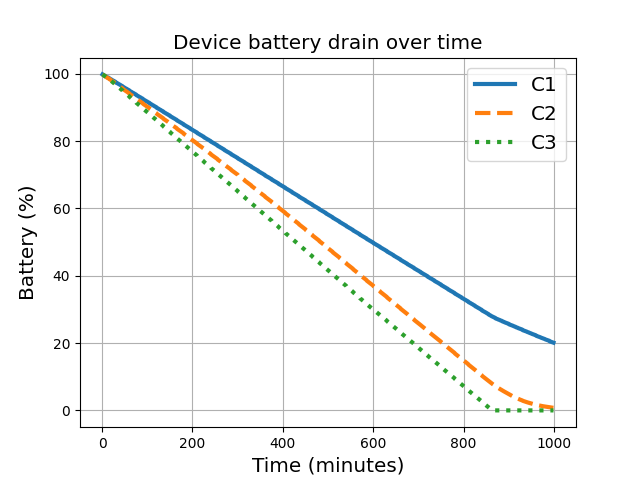
\includegraphics[width = \textwidth]{aggregatedBattery.png}
        \caption{Devices Battery Drain}
        \label{subfig:aggregates_battery}
    \end{subfigure}
    \begin{subfigure}{.35\textwidth}
        \centering
        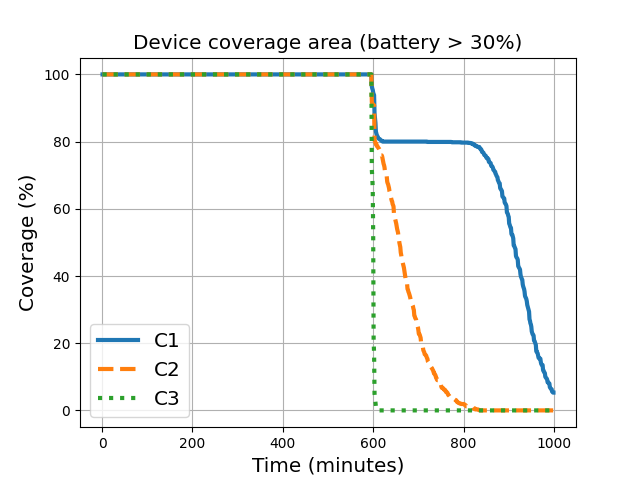
\includegraphics[width = \textwidth]{aggregatedCoverage.png}
        \caption{Devices Coverage}
        \label{subfig:aggregates_coverage}
    \end{subfigure}
    \begin{subfigure}{.35\textwidth}
        \centering
        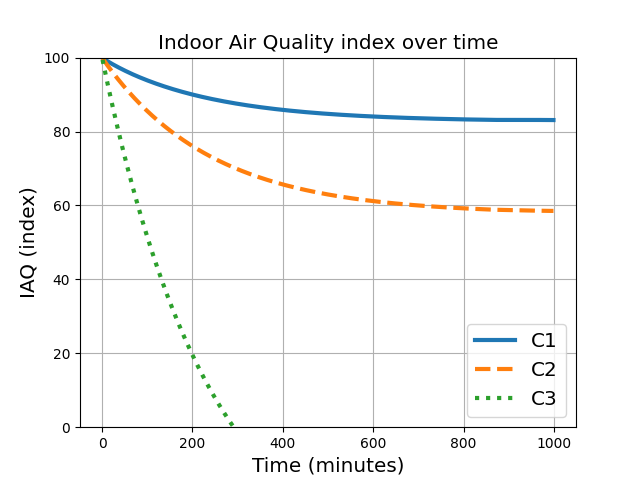
\includegraphics[width = \textwidth]{aggregatedIAQ.png}
        \caption{IAQ of the Building}
        \label{subfig:aggregates_iaq}
    \end{subfigure}
    \caption{Simulation aggregates of the three case scenarios}
    \label{fig:aggregates}
\end{figure}

Figure~\ref{fig:aggregates} shows the aggregated results of the three measures we captured during the simulations.
%
Each graph includes how the measure evolves under the three case scenarios.
%
Considering \emph{C1}, we see that the average battery of this scenario, shown in Figure~\ref{subfig:aggregates_battery}, drains more slowly than the other two cases. The light flexion around 850 minutes is due to the savings policy discussed in the specification.
%
Of course, as the number of persons increases, the battery drain curve is lower.
%
The coverage shown in Figure~\ref{subfig:aggregates_coverage} reflects the behaviour of the battery drainage.
%
As the time reaches 600 minutes, we can see that, for \emph{C3}, the average battery is lower than or equal to 30\%, which means that the minimal condition of the coverage can't be met: that is why we see in the coverage graph that the related curve drops abruptly.
%
The IAQ index presented in Figure~\ref{subfig:aggregates_iaq} evolves in the same way as the previous trends.
%
Generally, the IAQ index stabilises over time.
%
The steepness of the trend is influenced by the number of \lstinline{Human} agents. 
%
As our model only considers the number of people to calculate the CO$_2$ in a room, it is clear that the more people are present (and spend time in a room), the less time each room has to ventilate.
Each room, and generally the building, has no time to ventilate. 
%
In fact, if we consider the \emph{C3} trend line, we see that the IAQ index is dangerously low (even going below zero) while \emph{C1} and \emph{C2} present acceptable air quality levels.


\subsection{Using the Trace Command}\label{subsec:usingtrace}

We can gain insight into the individual simulation runs for each agent using the \emph{Trace} command.
%
This command was originally implemented to capture the movement of agents inside a physical environment. Indeed, the related specification includes the XYZ axes and attributes that represent the direction and the physical format.
%
However, we can exploit this by assigning the attributes from the IAQ scenario specification, i.e. \lstinline{x = batteryPerc;} and \lstinline{y = registeredIAQ;}.
The latter instructions are saved in a special file (\lstinline{iaq.trc}) used by different commands. Here, unlike in the simulation, we run a single \emph{replica}, so we do not use \lstinline{set_replica}. The main change is on command \lstinline{sr.trace} rather than \lstinline{sr.simulate}, which also requires the trace file rather than the simulation file.

The use of the \emph{Trace} command enables us to observe the device's battery behaviour and indoor air quality under different scenarios. 
%
We decided to consider different scenarios with high, medium, and low population density representing \emph{Main Hall} (Fig.~\ref{fig:mainHallCases}), \emph{Smaller Hall} (Fig.~\ref{fig:smallHallCases}), and \emph{Office Room} (Fig.~\ref{fig:officeCases}).
%
It is possible to observe in the \emph{C1} that, also with a low population density (10 humans) in the environment, the \emph{Main Hall} (Fig.~\ref{subfig:mainhallC1}) and the \emph{Small Hall} (Fig.~\ref{subfig:smallhallC1}) present air quality degradation.
%
The motivation is associated with the configuration of the rooms, which function as passageways facilitating movement between different areas. This configuration differs from that of an \emph{Office Room} (Fig.~\ref{subfig:officeC1}), which maintains good air quality over time with a low-density population.
%
In a scenario with 20 humans in the environment (\emph{C2}), the \emph{Office room} (Fig.~\ref{subfig:officeC2}) maintains almost good air quality, with a slight degradation over time. 
%
The \emph{Small Hall} (Fig.~\ref{subfig:smallhallC2}) presents a high increase of CO$_2$ inside the room that decreases the quality of the air, but it is not as drastic as the situation exhibited in the \emph{Main Hall} (Fig.~\ref{subfig:mainhallC2}), where the quality of the air decreases faster.
%
The last scenario (\emph{C3}) presents an exaggeration in which a high-density population of 60 humans is present in the environment. It is possible to observe how the \emph{Main Hall} and \emph{Small Hall} (Figs.~\ref{subfig:mainhallC3} and~\ref{subfig:smallhallC3}) curve is steep, and the air quality decreases fast.
%
In contradistinction to the other rooms, the \emph{Office Room} (Fig.~\ref{subfig:officeC3}) exhibits a less precipitous curve and nevertheless attains a hazardous index of IAQ.


\begin{figure}[!htbp]
    \centering
    \begin{subfigure}{.32\textwidth}
        \centering
        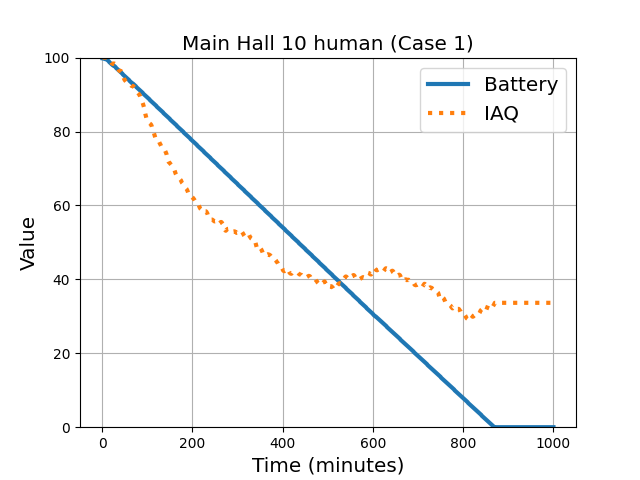
\includegraphics[width = \textwidth]{mainHall10HumanCase1.png}
        \caption{Case 1}
        \label{subfig:mainhallC1}
    \end{subfigure}
    \begin{subfigure}{.32\textwidth}
        \centering
        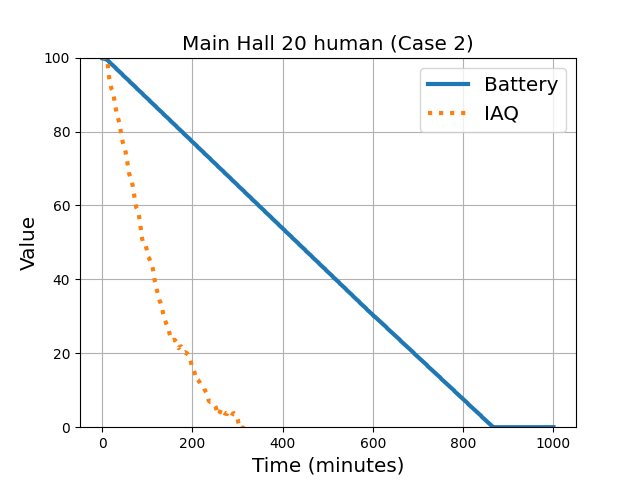
\includegraphics[width = \textwidth]{mainHall20HumanCase2.png}
        \caption{Case 2}
        \label{subfig:mainhallC2}
    \end{subfigure}
    \begin{subfigure}{.32\textwidth}
        \centering
        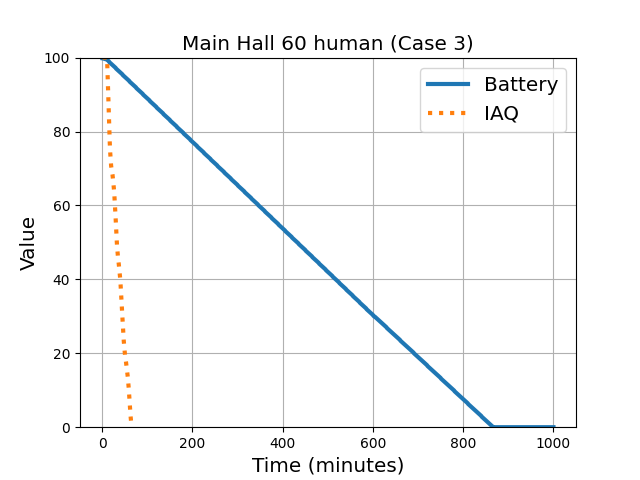
\includegraphics[width = \textwidth]{mainHall60HumanCase3.png}
        \caption{Case 3}
        \label{subfig:mainhallC3}
    \end{subfigure}
    \caption{Device Battery and IAQ of the Main Hall (Room 9)}
    \label{fig:mainHallCases}
\end{figure}

\begin{figure}[!htbp]
    \centering
    \begin{subfigure}{.32\textwidth}
        \centering
        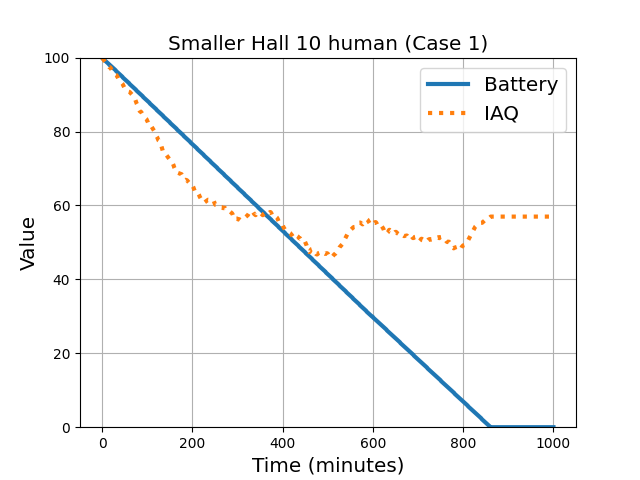
\includegraphics[width = \textwidth]{smallerHall10HumanCase1.png}
        \caption{Case 1}
        \label{subfig:smallhallC1}
    \end{subfigure}
    \begin{subfigure}{.32\textwidth}
        \centering
        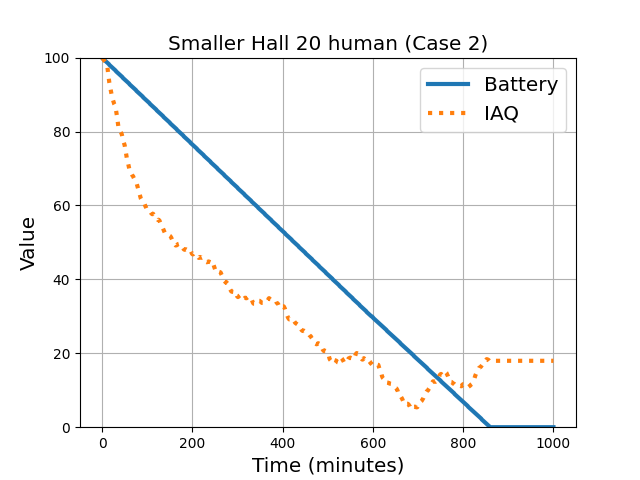
\includegraphics[width = \textwidth]{smallerHall20HumanCase2.png}
        \caption{Case 2}
        \label{subfig:smallhallC2}
    \end{subfigure}
    \begin{subfigure}{.32\textwidth}
        \centering
        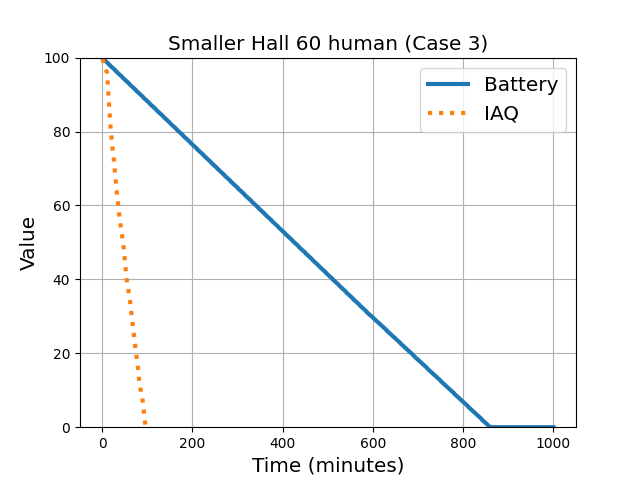
\includegraphics[width = \textwidth]{smallerHall60HumanCase3.png}
        \caption{Case 3}
        \label{subfig:smallhallC3}
    \end{subfigure}
    \caption{Device Battery and IAQ of the Smaller Hall (Room 5)}
    \label{fig:smallHallCases}
\end{figure}

\begin{figure}[!htbp]
    \centering
    \begin{subfigure}{.32\textwidth}
        \centering
        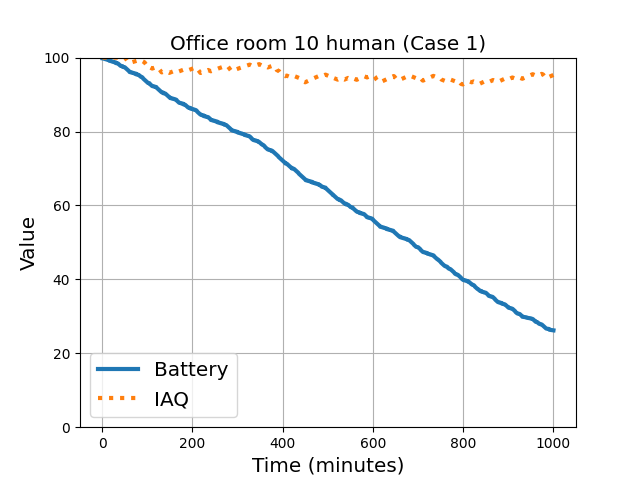
\includegraphics[width = \textwidth]{officeRoom10HumanCase1.png}
        \caption{Case 1}
        \label{subfig:officeC1}
    \end{subfigure}
    \begin{subfigure}{.32\textwidth}
        \centering
        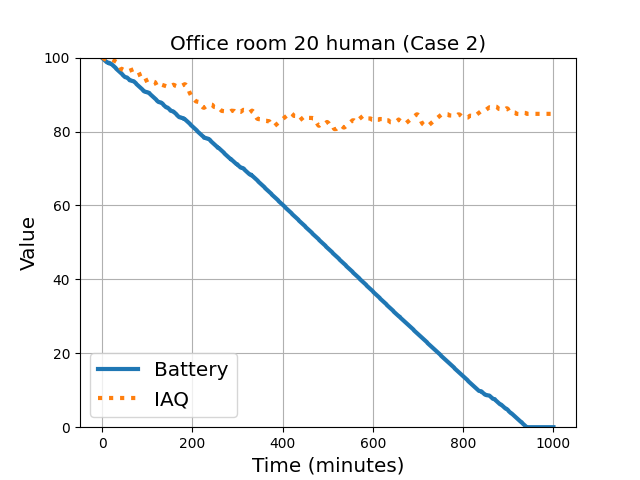
\includegraphics[width = \textwidth]{officeRoom20HumanCase2.png}
        \caption{Case 2}
        \label{subfig:officeC2}
    \end{subfigure}
    \begin{subfigure}{.32\textwidth}
        \centering
        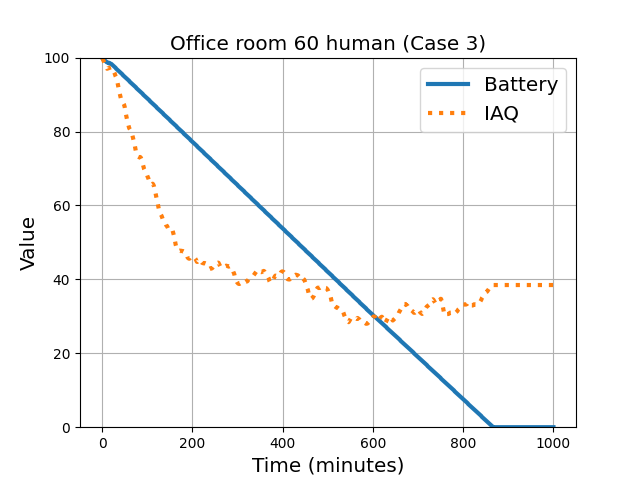
\includegraphics[width = \textwidth]{officeRoom60HumanCase3.png}
        \caption{Case 3}
        \label{subfig:officeC3}
    \end{subfigure}
    \caption{Device Battery and IAQ of the Office Room (Room 0)}
    \label{fig:officeCases}
\end{figure}

\subsection{Final remarks}\label{subsec:discussionApproach}

The results presented in the previous sections show that as the number of people in the environment increases, battery life decreases rapidly. Furthermore, a lower IAQ threshold, which triggers more frequent pollution readings, significantly increases the devices' overall energy consumption.
%
Coverage, defined as the percentage of devices retaining more than 30\% of their battery life, showed a consistent pattern across all cases. It has an initial stable phase followed by a first noticeable decline around a coverage of 80\%. This marks the first time the battery has fallen below the threshold.
%
In scenarios with the highest population density (60 humans), coverage degrades continuously, ultimately reaching complete absence. In contrast, scenarios exhibiting lower population density demonstrate a more gradual decline.
%
Notably, the case with 20 humans experienced a temporary slowdown in coverage loss before dropping sharply.
%
In contrast, the lower-density population case (10 humans) exhibited stable coverage close to 80\% for most of the observed time window, without reaching zero.
%
The building's IAQ shows how strongly it is influenced by population density. The first two cases, with low- and moderate-density populations of 10 and 20 humans, show a moderate decrease in air quality.
%
Conversely, in the third case, where 60 humans are present, it is evident that a high-density population significantly increases CO$_2$ concentration in the rooms. This phenomenon leads to a significant deterioration in air quality and a substantial decline in IAQ.
%
These considerations demonstrate how our approach can be a useful tool for informing and guiding decision-making during the design phase of an IoT environment.
%
By analysing the evolution of the simulated scenario, we can avoid deploying the scenario in the real world.
%
Additionally, the proposed approach allows us to scale it up to more complex scenarios, or even unexpected ones (as in the case of 60 people).

We can finally observe that all the analyses presented in this paper can be completed in a reasonable amount of time. Indeed, Figure~\ref{fig:simulationtime} shows that if we increase the number of rooms, the simulation time increases linearly. 


\begin{figure}[tbp]
\begin{center}
    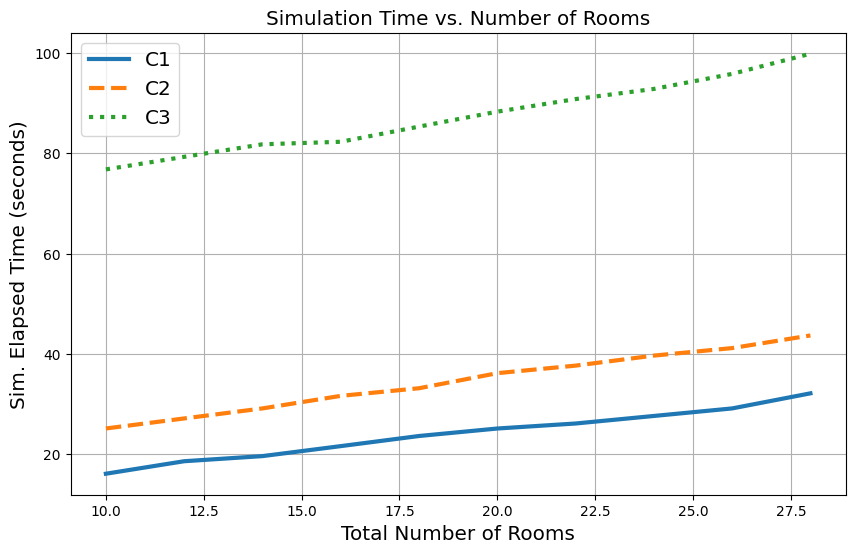
\includegraphics[width = 0.5\textwidth]{simvsrooms.png}
    \caption{Simulation Time}
    \label{fig:simulationtime}
    \end{center}
\end{figure}



\section{Conclusions and Future Work}\label{sec:conc}

In this paper, we analysed the evolution of a smart IoT ecosystem designed for IAQ monitoring and simulated within a university-inspired building environment. This was achieved using the \yoda{} MAS language and the \sibilla{} simulation tool.

We plan to extend our work in two different directions. First, we aim to further improve the model. As of now, the proposed scenario is an example of how \yoda{} can be used to design an IoT ecosystem more abstractly.
%
However, we can further increase the model's complexity (and precision) by accounting for more details about room locations and capacities, or by considering different people's movement patterns in the building. 
%
To simplify this task, we plan to extend \yoda{} with new primitives and constructs specifically thought to describe and constrain the movement of agents over a physical space. 

Moreover, we plan to integrate the proposed model into a monitoring system that can compare real data collected from a building with simulation-generated data. 
%
This approach will allow us, on the one hand, to tune the model and evaluate its accuracy relative to the real system, and, on the other hand, to build a \emph{digital twin} that the monitor can use to anticipate unwanted or dangerous situations.
%
To tune the model, we plan to use parameter synthesis~\cite{MatteucciQL24} integrated in \sibilla{}, while unwelcome computations can be identified using formal tools for runtime verification.
%
Indeed, \sibilla{} integrates the \emph{GLoTL} temporal logic~\cite{glotl}, which allows us to determine whether the model satisfies properties at the global and local levels.
%
This tool can be used to determine whether, for example, the device's coverage is satisfied for a given period, or whether the IAQ in one of the rooms is acceptable over an interval.


\paragraph*{Acknowledgements} The authors thank the anonymous reviewers for their constructive comments and suggestions, which helped to improve the quality of this paper.

%
\bibliographystyle{splncs04}
\bibliography{bib}
%
\end{document}
